% Identify here the order in which you plan to implement the subcomponents of your system and the order in which you plan to integrate such subcomponents and test the integration.


\subsection{Overview}
\begin{flushleft}
To comply with standard design practices it is suggested to undergo unit testing as each component is built, integration testing as component get pieced together, and system testing to validate the system as a whole. This section will detail the order in which the components should be built, the method to carry out testing, and the manner in which to integrate the components.
\end{flushleft}

 
\subsection{Implementation Plan}
\begin{flushleft}
As stated previously, the entire system can be decomposed into 15 components which shall be built in the following order: 
\end{flushleft}

\begin{enumerate}
\item AuthenticationManager
\item FarmerReportManager
\item AgronomistReportManager
\item DataAggregationManager
\item StatisticsManager
\item DailyPlanManager
\item MessageManager
\item FarmManager
\item RankingManager
\item TriggerManager
\item NotificationManager
\item ForumManager
\item FarmerSuggestionManager
\item RecommenderManager
\item WeatherManager
\end{enumerate}

\begin{flushleft}
This ordering of components prioritizes the most important features expected by the DREAM system and core components that serve as a foundation or basis for other components. Namely, the \(\ll\)AuthenticationManager\(\gg\) is the first component to be built to emphasize the importance of security. Before any user can do anything they must be able to login. Then, components supporting the generation of reports and handling the data are listed. This is a core function of the DREAM system and the foundation of the value-add of the DREAM system. After that, additional components that generate more data and support the aggregation of diverse data sources, such as \(\ll\)DailyPlanManager\(\gg\), \(\ll\)MessageManager\(\gg\), and \(\ll\)FarmManager\(\gg\), are listed. These component just build on the core functionalities that have already been established. Then, the remaining components refine the features that the DREAM system provides and fulfill the goals committed to by the system. \\
\smallskip
These four phases are also shown in Figure \ref{fig:implementationPhases}. The components have been seperate in such a way so that when each phase is complete, the subsequent or precedent phase can be iterated over. For example, the \(\ll\)DataAggregationManager\(\gg\) and \(\ll\)StatisticsManager\(\gg\) are both included in Phase 1. The components in Phase 3, such as the \(\ll\)FarmManager\(\gg\), however, may offer more data to plug into the \(\ll\)DataAggragationManager\(\gg\) or may tie into elements built in Phase 1 such as the \(\ll\)DailyPlanManager\(\gg\) tying into the reports generated in the \(\ll\)AgronomistReportManager\(\gg\). The segmentation of the phases not only considers priority but also establishes reasonable points in the implementation effort to consider iterating over other components that may or may not have been built, yet. 
\end{flushleft}

\begin{figure}[hbt!]
\centering
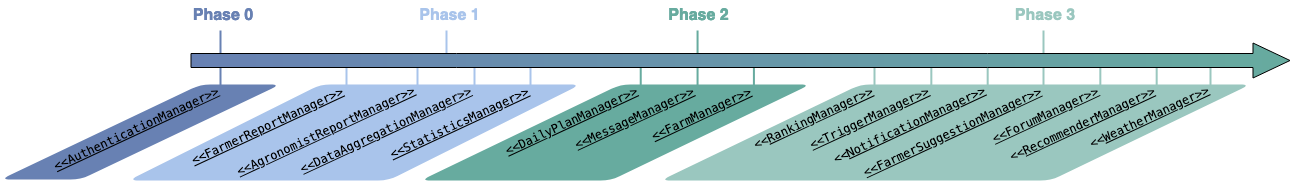
\includegraphics[width=\textwidth]{../images_diagrams/dd/implementation_phases.png}
\caption{Implementation Phases.}
\label{fig:implementationPhases}
\end{figure}


\subsection{Integration and Testing Plan}
\subsection{System Testing}